\documentclass[11pt]{report}
\usepackage{outline}
\usepackage[utf8]{inputenc}
\usepackage{graphicx}
\usepackage[top=1in,bottom=1in,left=1in,right=1in]{geometry}
\usepackage{wrapfig}
\usepackage[most]{tcolorbox}
\usepackage[colorlinks = true,
            linkcolor = blue,
            urlcolor  = blue,
            citecolor = blue,
            anchorcolor = blue]{hyperref}
%\usepackage{fancyhdr}
\usepackage{subcaption}
\usepackage{apacite}
\bibliographystyle{apacite}
\usepackage[toc,page]{appendix}
\usepackage{grffile}
\newcommand{\Lumi}{ \mathcal{L}}


\title{Analysis Note on the Deeply Virtual Neutral Pion Production Cross Section Measurement}


\author{Robert Johnston$^1$ \and Sangbaek Lee$^1$
\and Igor Korover$^1$
\and Xiaqing Li$^1$
\and Andrey Kim$^2$
}
\date{%
    $^1$Massachusetts Institute of Technology\\%
    $^2$University of Connecticut\\[2ex]%
    \today
}


\begin{document}

\maketitle
\tableofcontents
\cleardoublepage
% \phantomsection
\addcontentsline{toc}{chapter}{\listfigurename}
\listoffigures

\chapter{Collaborator's Note: Differences Between This and Prior Analysis Note}
For ease of reading by collaborators, here are a listing of differences between this analysis note (for Fall 2022 DNP meeting) and the most recently collaboration approved analysis note (for April 2022 APS meeting):
\begin{itemize}
    \item \textbf{Model Comparison} The large reported change from analysis notes is the inclusion of the Goloskov Kroll Model to compare the preliminary CLAS12 cross section to a theoretical model. This is covered in section \ref{chap:GKmodel}.
    \item \textbf{Exclusivity Cuts and Results} There are small improvements to this text for a more complete description of work accomplished.
\end{itemize}

\chapter{PID}

For this analysis all final state particles should be detected.
After $\pi^0$ decay we are going to have 4 particles: electron, proton and two photons.
The particle identification methods are applied to select the exclusive event with at least one electron, proton and two photons. 


\section{Electron, Proton, and Photon}
Basic event builder cuts are utilized, then additional cuts are made that are common with the RGA Analysis note (\href{https://www.overleaf.com/project/5ea737720942930001ff5e9c}{overleaf link} and developed by Sangbaek Lee (sangbaek@mit.edu - \href{https://github.com/Sangbaek/analysis_code/tree/analysis/pid}{github code here}. For this analysis, both the central detector and forward detector are utilized for proton tracking. The forward tagger is also utilized for photon identification. 



\section{Neutral pion}
In addition to individual particle PID procedures the cut on the mass of two photons is applied:
\begin{itemize}
	\item $0.07<M_{\gamma\gamma}<0.2$ GeV
\end{itemize}
The pion is more thoroughly constrained by the exclusivity cuts, described in the next section.


\begin{figure}[hbt]
	\centering
	\includegraphics[page=6,width=0.6\linewidth]{figures/eppi0.exclusive.pdf}
	
	\caption{The distribution for mass of two photons $M_{\gamma\gamma}$}.
	\label{fig:ggmass}
	
	\centering
	\includegraphics[page=6,width=0.6\linewidth]{pid_figs/Mpi0.png}
	
	\caption{The distribution for mass of two photons after exclusivity cuts}.
	\label{fig:ggmass_after}
	
\end{figure}



\chapter{Exclusive Selection}  
\label{chap:exclusive}
\section{Exclusive distributions}


\begin{wrapfigure}{r}{0.58\textwidth}
	\vspace*{-0.3cm}
	\includegraphics[page=10,width=0.97\linewidth]{figures/eppi0.exclusive.pdf}
	\caption{MM$^2$ (epX) vs $\theta_X\pi$ 2D distribution.}
	\label{fig:MM2vsThetaXPi}
\end{wrapfigure}
After the selection of events with at least one electron, proton and two photons, it is time to take a look at the exclusive distributions.
The Fig.~\ref{fig:MM2vsThetaXPi} shows 2D distribution of MM$^2$ (epX) vs $\theta_{X\pi}$, where MM$^2$ (epX) is a missing mass squared of (epX) system and should have a peak near 0.0182 GeV$^2$, and $\theta_{X\pi}$ is an angle between expected and reconstructed pion.
The bright spot on the figure corresponds to the exclusive $ep\rightarrow~ep\pi^0$ events.
In order to reduce the background exclusivity cuts  need to be developed based on the conservation of energy and momentum.
The relevant 1D exclusive distributions are shown on the Fig.~\ref{fig:rawexclusive1} and \ref{fig:rawexclusive2}.

\begin{figure}[hbt]
	\centering
	\includegraphics[page=4,width=0.47\linewidth]{figures/eppi0.exclusive.pdf}
	\includegraphics[page=5,width=0.47\linewidth]{figures/eppi0.exclusive.pdf}

	\caption{Exclusive distributions for events with at least one electron, proton and two photons.}
	\label{fig:rawexclusive1}
\end{figure}

\begin{figure}[hbt]
	\centering
	\includegraphics[page=6,width=0.47\linewidth]{figures/eppi0.exclusive.pdf}
	\includegraphics[page=8,width=0.47\linewidth]{figures/eppi0.exclusive.pdf}
	
	\caption{Exclusive distributions for events with at least one electron, proton and two photons.}
	\label{fig:rawexclusive2}
\end{figure}

\subsection{Tight $M_{\gamma\gamma}$ mass and transverse missing momenta cuts}

The first step is to use tighter $\gamma\gamma$ mass cut: $0.096<M_{\gamma\gamma}<0.168$ GeV, and take a look at the missing transverse momentum distributions (see Fig.~\ref{fig:ptdistributions}).
From momentum conservation law we expect transverse momentum to be zero, so we can apply cuts on $\Delta p_x$ and $\Delta p_y$ to further improve exclusive channel selection.
The cuts $|\Delta p_x|<0.2$ and $|\Delta p_y|<0.2$ correspond roughly to 4-5 $\sigma$.

\begin{figure}[hbt]
	\centering
	\includegraphics[page=24,width=0.47\linewidth]{figures/eppi0.exclusive.pdf}
	\includegraphics[page=25,width=0.47\linewidth]{figures/eppi0.exclusive.pdf}
	
	\caption{Exclusive distributions for events with at least one electron, proton and two photons.}
	\label{fig:ptdistributions}
\end{figure}

The exclusive distributions after tight $M_{\gamma\gamma}$ mass and transverse missing momenta cuts are shown on Fig.~\ref{fig:rawexclusive3} and display much stronger signal peaks on top of reduced background.

\begin{figure}[hbt]
	\centering
	\includegraphics[page=43,width=0.45\linewidth]{figures/eppi0.exclusive.pdf}
	\includegraphics[page=44,width=0.45\linewidth]{figures/eppi0.exclusive.pdf}
	
	\includegraphics[page=45,width=0.45\linewidth]{figures/eppi0.exclusive.pdf}
    \includegraphics[page=47,width=0.45\linewidth]{figures/eppi0.exclusive.pdf}

	\caption{Exclusive distributions after tight $M_{\gamma\gamma}$ mass and transverse missing momenta cuts .}
	\label{fig:rawexclusive3}
\end{figure}

\subsection{$\theta_{X\pi}$ cut determination}

The cut on angle between expected and reconstructed pion is used in order to further reduce background.
To choose the value of the $\theta_{X\pi}$ cut the $MM^2(epX)$ distribution is analyzed at multiple $\theta_{X\pi}$ cut values and fit using gaussian+polynomial function as shown on Fig.~\ref{fig:mm2fordifferenttheta}.
From the fit we can estimate the number of good exclusive events (gaussian) and the number of background events (polynomial) and their dependence on $\theta_{X\pi}$ cut.
Fig.~\ref{fig:sigbgvsthetacutQ2} and~\ref{fig:sigbgvsthetacutxB} show the numbers of signal and background events as functions of $\theta_{X\pi}$ cut value for multiple bins in $Q^2$ and $x_B$.
These plots show that the cut $\theta_{X\pi}<2^\circ$ allows to select the most number of good events with the least background, and relaxing it beyond $2^\circ$ does not gain us any good exclusive events but increases background.


\begin{figure}[hbt]
	\centering
	\includegraphics[page=123,width=0.3\linewidth]{figures/sigbg_eppi0.pdf}
	\includegraphics[page=125,width=0.3\linewidth]{figures/sigbg_eppi0.pdf}
	\includegraphics[page=128,width=0.3\linewidth]{figures/sigbg_eppi0.pdf}
	
	\includegraphics[page=130,width=0.3\linewidth]{figures/sigbg_eppi0.pdf}
	\includegraphics[page=133,width=0.3\linewidth]{figures/sigbg_eppi0.pdf}
	\includegraphics[page=135,width=0.3\linewidth]{figures/sigbg_eppi0.pdf}
	
	\caption{$MM^2(epX)$ distributions for multiple $\theta_{X\pi}$ cut values.}
	\label{fig:mm2fordifferenttheta}
\end{figure}


\begin{figure}[hbt]
	\centering
	
	\includegraphics[width=0.32\linewidth,page=34]{figures/sigbg_eppi0.pdf}
	\includegraphics[width=0.32\linewidth,page=51]{figures/sigbg_eppi0.pdf}
	\includegraphics[width=0.32\linewidth,page=68]{figures/sigbg_eppi0.pdf}
	
	\includegraphics[width=0.32\linewidth,page=85]{figures/sigbg_eppi0.pdf}
	\includegraphics[width=0.32\linewidth,page=102]{figures/sigbg_eppi0.pdf}
	\includegraphics[width=0.32\linewidth,page=119]{figures/sigbg_eppi0.pdf}
	
	\caption{The numbers of signal (red markers) and background (black markers) events as functions of $\theta_{X\pi}$ cut value for multiple $Q^2$ bins.}
	\label{fig:sigbgvsthetacutQ2}
\end{figure}


\begin{figure}[hbt]
	\centering
	
	\includegraphics[width=0.32\linewidth,page=136]{figures/sigbg_eppi0.pdf}
	\includegraphics[width=0.32\linewidth,page=153]{figures/sigbg_eppi0.pdf}
	\includegraphics[width=0.32\linewidth,page=170]{figures/sigbg_eppi0.pdf}
	
	\includegraphics[width=0.32\linewidth,page=187]{figures/sigbg_eppi0.pdf}
	\includegraphics[width=0.32\linewidth,page=204]{figures/sigbg_eppi0.pdf}
	
	\caption{The numbers of signal (red markers) and background (black markers) events as functions of $\theta_{X\pi}$ cut value for multiple $x_B$ bins.}
	\label{fig:sigbgvsthetacutxB}
\end{figure}

\clearpage

\subsection{Final exclusivity cuts}

The list of final exclusive cuts is following:
\begin{itemize}
	\item $\Delta p_x<0.2$ GeV
	\item $\Delta p_y<0.2$ GeV
	\item $\theta_{X\pi}<2^\circ$
	\item $0.096<M_{\gamma\gamma}<0.168$ GeV
	\item $MM^2(epX)<0.5$ GeV$^2$
\end{itemize}

Exclusive distributions after all exclusivity cut except $MM^2(epX)<0.5$ GeV are shown on Fig.~\ref{fig:finalexclusive}

\begin{figure}[hbt]
	\centering
	
	\includegraphics[page=82,width=0.32\linewidth]{figures/eppi0.exclusive.pdf}
	\includegraphics[page=83,width=0.32\linewidth]{figures/eppi0.exclusive.pdf}
	\includegraphics[page=84,width=0.32\linewidth]{figures/eppi0.exclusive.pdf}
	\caption{Exclusive distributions after all exclusivity cuts .}
	\label{fig:finalexclusive}
\end{figure}



\chapter{Simulations}
\label{chap:acc}
\iffalse
NOTES TO SELF:
physics motivation
data sets before event selection
PID
exclusive cuts
results to show
1 slide of what needs to go from here to cross section
\fi

\section{Generator and Simulations}
    Simulations are necessary in order to extract correction factors. Presently, only an acceptance correction using a non-radiative generator has been calculated; other correction factors are forthcoming but will not be including in this note. 

    GEMC was used to process generated events through the CLAS12 fall 2018 RG-A configuration. Specifically, a generator based off the GK model and CLAS6 data - aao\_norad\footnote{https://github.com/drewkenjo/aao\_norad}. 
    

\section{Comparison to Data: Missing Mass Distributions}

The standard aao simulations result in missing mass distributions that are too optimistic compared to experimental data. Observe the discrepancies between simulated and experimental distributions in figure \ref{fig:bad}. 


\begin{figure}[hbt]
	\centering
	\includegraphics[page=125,width=0.3\linewidth]{simcomp/nosmear/outbending_rad_All_All_All_no_smearingME_epgg_exp_vs_sim.png}
	\includegraphics[page=123,width=0.3\linewidth]{simcomp/nosmear/outbending_rad_All_All_All_no_smearingMM2_egg_exp_vs_sim.png}
	\includegraphics[page=128,width=0.3\linewidth]{simcomp/nosmear/outbending_rad_All_All_All_no_smearingMM2_epgg_exp_vs_sim.png}
	\includegraphics[page=130,width=0.3\linewidth]{simcomp/nosmear/outbending_rad_All_All_All_no_smearingMM2_ep_exp_vs_sim.png}
	\includegraphics[page=133,width=0.3\linewidth]{simcomp/nosmear/outbending_rad_All_All_All_no_smearingMpi0_exp_vs_sim.png}
	\includegraphics[page=135,width=0.3\linewidth]{simcomp/nosmear/outbending_rad_All_All_All_no_smearingMPt_exp_vs_sim.png}
	
	\caption{Comparison of experiment (blue) and simulation (red) missing mass, energy, momentum, and invariant gamma-gamma mass distributions, before any smearing factors were added to the simulation data.}
	\label{fig:bad}
\end{figure}



To improve the matching between simulation and experiment, gaussian smearing factors were added after reconstruction to the simulated dataset. These factors were tuned by Sangbaek Lee to have optimal matching across all missing mass spectra combinations (figure \ref{fig:good}. Once these factors were determined, the simulations were used to extract an acceptance correction.


\begin{figure}[hbt]
	\centering
	\includegraphics[page=125,width=0.3\linewidth]{simcomp/yessmear/outbending_rad_All_All_All_for_aps_2022_plots_sangcutsME_epgg_exp_vs_sim.png}
	\includegraphics[page=123,width=0.3\linewidth]{simcomp/yessmear/outbending_rad_All_All_All_for_aps_2022_plots_sangcutsMM2_egg_exp_vs_sim.png}
	\includegraphics[page=128,width=0.3\linewidth]{simcomp/yessmear/outbending_rad_All_All_All_for_aps_2022_plots_sangcutsMM2_epgg_exp_vs_sim.png}
	\includegraphics[page=130,width=0.3\linewidth]{simcomp/yessmear/outbending_rad_All_All_All_for_aps_2022_plots_sangcutsMM2_ep_exp_vs_sim.png}
	\includegraphics[page=133,width=0.3\linewidth]{simcomp/yessmear/outbending_rad_All_All_All_for_aps_2022_plots_sangcutsMpi0_exp_vs_sim.png}
	\includegraphics[page=135,width=0.3\linewidth]{simcomp/yessmear/outbending_rad_All_All_All_for_aps_2022_plots_sangcutsMPt_exp_vs_sim.png}
	
	\caption{Comparison of experiment (blue) and simulation (red) missing mass, energy, momentum, and invariant gamma-gamma mass distributions, with smearing factors added to the simulation data proton and photon momenta.}
	\label{fig:good}
\end{figure}


\section{Acceptance Correction}

The acceptance correction, in each kinematic bin, was simply calculated as $\frac{N_{rec}}{N_{gen}}$, where $N_{gen}$ is the number of events produced by the generator in a specific bin, and $N_{rec}$ is the number of events in that bin that were reconstructed and identified as a $DV\pi^0P$ event by exclusivity cuts. 

Low acceptance bins (less than 5\%) were excluded from further study, following from the CLAS6 analysis procedure. 

\chapter{Luminosity and Virtual Photon Flux Factor}
\label{chap:lumi}
\section{Luminosity}

Luminosity is calculated according to equation \ref{lumieq}
 \begin{equation}\label{lumieq}
            \Lumi = \frac{N_A l \rho Q_{FCUP}}{e}
\end{equation}

The terms in equation \ref{lumieq} are as tabulated in table \ref{lumitable}. The accumulated charge on the Faraday cup is calculated by taking difference between the maximum and minimum values of beamQ for each run, and then summing these values. The luminosity determined for the fall 2018 inbending run was 5.5E+40 cm$^{-2}$ and the fall 2018 outbending run was 4.65E+40 cm$^{-2}$

\begin{table}[h]
    \centering
    \begin{tabular}{rcc}
         %& Heading 1 & Heading 2 \\\hline
        Quantity &  & CLAS12 Value \\\hline
       Avogadro's Number &  N$_A$  & $6x10^{23}$ \\
        Electron Charge &e  &  $1.6x10^{-19}$ \\
        Target Length &l &  5 cm \\
        Target Density &$\rho$  &  0.07 $g/cm^3$ (LH2) \\
        Charge on Faraday Cup & $Q_{FCUP}$ &  In data\\
    \end{tabular}
\caption{Terms of Luminosity Equation}
\end{table}\label{lumitable}

\section{Virtual Photon Flux Factor}
To calculate the reduced cross sections, it is necessary to calculate the virtual photon flux factor, $\Gamma (Q^2, x_B, E)$, which was calculated for each bin using equation \ref{gamma1}:

 \begin{equation}\label{gamma1}
            \Gamma (Q^2, x_B, E) = \frac{\alpha}{8\pi} \frac{Q^2}{m^2_pE^2}\frac{1-x_B}{x_B}\frac{1}{1-\epsilon}
\end{equation}

$\alpha$ is the fine structure constant, E is the beam energy, and $\epsilon$ is calculated using equation \ref{gamma2}

 \begin{equation}\label{gamma2}
            \epsilon = \frac{1-y-\frac{Q^2}{4E^2}}{1-y+\frac{y^2}{2}+\frac{Q^2}{4E^2}}
\end{equation}

For each bin, y is calculated using equation \ref{gamma3}, using the average value of $Q^2$ and $x_B$ in each bin.

 \begin{equation}\label{gamma3}
           y = \frac{\omega}{E} = \frac{Q^2}{2x_Bm_pE}
\end{equation}

\chapter{Results}
\section{Reduced Cross Section}

The experimental cross section is given by equation \ref{xsec}

 \begin{equation}\label{xsec}
     \frac{d^4\sigma_{\gamma^*p \rightarrow p'\pi^0}}{dQ^2dx_Bdtd\phi_{\pi}} = \frac{N(Q^2,x_B,t,\phi_{\pi})}{\Lumi_{int}\Delta Q^2\Delta x_B\Delta t\Delta \phi} \frac{1}{\epsilon_{ACC} \delta_{RC} \delta_{Norm} Br(\pi^0 \rightarrow \gamma \gamma)}
\end{equation}

$N(Q^2,x_B,t,\phi_{\pi})$ is the raw number of events in a specific kinematic bin and is calculated as described in chapter \ref{chap:exclusive}. $\Lumi_{int}$ is the integrated luminosity over the run of the experiment under analysis and is calculated as described in chapter \ref{chap:lumi}.$\Delta Q^2\Delta x_B\Delta t\Delta \phi$ are the bin widths for the 4 kinematic binning variables. $\epsilon_{ACC}$ is the acceptance correction, and is calculated as described in chapter \ref{chap:acc}. $\delta_{RC} \delta_{Norm} Br(\pi^0 \rightarrow \gamma \gamma)$ are the radiative, overall, and branching ratio correction factors, and are not yet included in this cross section calculation. 
\\~\\
Initial investigations show that radiative corrections will be on the order of 5\%, the branching ratio is a 1.2\% correction, and the overall normalization is not yet determined but was 10\% for the CLAS6 experiment; we expect the CLAS12 experiment overall normalization will be similar or less in magnitude. Thus, all of these corrections are much smaller than the acceptance correction, and will be included in future work but are not critical for preliminary analysis work.

The accepted results from the CLAS6 experiment \cite{Bedlinskiy2014} can be used as a cross check for this work. Published values for the reduced cross sections from the CLAS6 experiment for the DV$\pi^0$P channel are available \href{https://journals.aps.org/prc/supplemental/10.1103/PhysRevC.90.025205}{here}. To calculate the reduced cross sections, we divide the cross section as described in equation \ref{xsec} by the virtual photon flux factor $\Gamma$ for each kinematic bin, where $\Gamma$ is calculated as described in chapter \ref{chap:lumi}. The reduced cross section is then given by equation \ref{xsec_red}.

 \begin{equation}\label{xsec_red}
    \frac{d^2\sigma_{\gamma^*p \rightarrow p'\pi^0}(Q^2,x_B,t,\phi_{\pi},E)}{dtd\phi} = \frac{1}{\Gamma_V(Q^2,x_B,E)} \frac{d^4\sigma_{\gamma^*p \rightarrow p'\pi^0}}{dQ^2dx_Bdtd\phi_{\pi}}
\end{equation}


 \begin{equation}\label{xsec_red_full}
    \frac{d^2\sigma_{\gamma^*p \rightarrow p'\pi^0}}{dtd\phi} = \frac{1}{\Gamma_V(Q^2,x_B,E)} \frac{N(Q^2,x_B,t,\phi_{\pi})}{\Lumi_{int}\Delta Q^2\Delta x_B\Delta t\Delta \phi} \frac{1}{\epsilon_{ACC} \delta_{RC} \delta_{Norm} Br(\pi^0 \rightarrow \gamma \gamma)}
\end{equation}
Some plots of reduced cross section for CLAS12 outbending Fall 2018 dataset are shown in figure \ref{fig:reduced_xsec_plots}. The cross sections show good agreement with the published CLAS6 results. The outbending dataset is contains mostly lower $Q^2$ events and the inbending dataset is not yet properly analyzed, so higher $Q^2$ comparisons are not avaliable for this analysis note. 


\begin{figure}[hbt]
	\centering
	\includegraphics[page=125,width=0.3\linewidth]{reduced_xsecs/ReducedCrossSectionFitOverPhi_Q2175_x_B022_t03.png}
	\includegraphics[page=123,width=0.3\linewidth]{reduced_xsecs/ReducedCrossSectionFitOverPhi_Q2175_x_B022_t12.png}
	\includegraphics[page=128,width=0.3\linewidth]{reduced_xsecs/ReducedCrossSectionFitOverPhi_Q2175_x_B022_t17.png}
	\includegraphics[page=130,width=0.3\linewidth]{reduced_xsecs/ReducedCrossSectionFitOverPhi_Q2138_x_B017_t12.png}
	\includegraphics[page=133,width=0.3\linewidth]{reduced_xsecs/ReducedCrossSectionFitOverPhi_Q2187_x_B027_t05.png}
	\includegraphics[page=135,width=0.3\linewidth]{reduced_xsecs/ReducedCrossSectionFitOverPhi_Q2195_x_B031_t05.png}
	
	\caption{Comparison of CLAS12 (blue) and CLAS6 (red) reduced cross sections, using Fall 2018 outbending dataset. Error bars are statistical only.}
	\label{fig:reduced_xsec_plots}
\end{figure}

To compare these results, we can examine the form of the differential cross section, under the single photon exchange assumption we can write the differential cross section as in equation \ref{eq:dif1}

 \begin{equation}\label{dif1}
     \frac{d^4\sigma_{\gamma^*p \rightarrow p'\pi^0}}{dQ^2dx_Bdtd\phi_{\pi}} =
     \Gamma (Q^2, x_B, E)
     \frac{1}{2\pi}
     ((\frac{d\sigma_T}{dt}+\epsilon\frac{d\sigma_L}{dt})+
     \epsilon cos(2\phi) \frac{d\sigma_{TT}}{dt} + \sqrt{2\epsilon(1+\epsilon)}cos(\phi)\frac{d\sigma_{LT}}{dt})
\end{equation}

Where $\Gamma (Q^2, x_B, E)$ is the virtual photon flux, give in equation \ref{gamma1}
 \begin{equation}\label{gamma1}
            \Gamma (Q^2, x_B, E) = \frac{\alpha}{8\pi} \frac{Q^2}{m^2_pE^2}\frac{1-x_B}{x_B^3}\frac{1}{1-\epsilon}
\end{equation}

The reduced cross section terms then are just functions of the structure functions and epsilon. At these kinematics, epsilon is approximately 0.5 for the CLAS6 data and 0.9 for the CLAS12 datasets, but given that the $((\frac{d\sigma_T}{dt}+\epsilon\frac{d\sigma_L}{dt})$ dominates the cross section, these differences are minor. Therefore, close (but not exact) agreement between the two datasets for given kinematic bins are expected for the reduced cross sections. More quantitative statements will be made in coming months, but not at this point.


\section{T Dependence of Cross Section}

We can calculate the t dependence of the differential cross section $d\sigma_U/dt$ by integrating the reduced cross sections over $\phi$ as in equation \ref{eq:tdep}

 \begin{equation}\label{eq:tdep}
    \frac{d\sigma_U}{dt} = \int \frac{d^2\sigma}{dtd\phi} d\phi
\end{equation}

In order to account for regions where the detectors used in CLAS6 and CLAS12 have zero acceptance, it is necessary to include a correction factor $\eta'$, defined in equation \ref{eq:eta} and calculated using Monte Carlo. 

 \begin{equation}\label{eq:eta}
    \eta' = \frac{\int_{\Omega*} \frac{d^2\sigma}{dtd\phi} }{\int_{\Omega} \frac{d^2\sigma}{dtd\phi}}
\end{equation}

However, at this point this correction factor has not yet been calculated. Instead, we can focus on kinematic bins where the coverage in $\phi$ is nearly 100\%, such that $\eta'$ would be small. In figure \ref{fig:tdep} we show the t dependent cross section, calculated only for bins where the coverage in $\phi$ was greater than 90\%, thus the error from not including the $\eta'$ correction factor is only approximately 10\%. We observe a good agreement in the b slope parameter, which describes the width of the transverse momentum distribution of the proton, between CLAS12 and the published CLAS6 data.


\begin{figure}[hbt]
	\centering
	\includegraphics[page=125,width=0.45\linewidth]{tdep/fig_1.0_0.15.png}
	\includegraphics[page=130,width=0.45\linewidth]{tdep/fig_1.5_0.15.png}

	\caption{CLAS12 and CLAS6 t dependence of cross sections. The fits are exponential functions $Ae^{-bt}$, where the slope parameter b are in close agreement for the bins considered. The overall normalization A is not yet determined for the CLAS12 dataset, so a small overall offset from the CLAS6 data is expected. Errors are only statistical.}
	\label{fig:tdep}
\end{figure}


\chapter{Comparison with Model} 
\label{chap:GKmodel}
\section{GK Model}

We compare the preliminary cross section to the model developed by S.V. Goloskokov and P. Kroll \cite{Goloskokov2010}. This model uses the handbag model to produce theoretical curves for specified sets of kinematic points. This model was implemented in the PARTONS framework \cite{Berthou2018} and was also used in the published CLAS6 result to compare with their experimental cross section, reproduced below in figure \ref{fig:oldres} \cite{Bedlinskiy2014}.

\begin{figure}[hbt]
	\centering
	\includegraphics[page=6,width=0.6\linewidth]{clas6comp.jpg}
\end{figure}\label{fig:oldres}

To validate the model, we ran the implementation to generate curves and compared to the published CLAS6 result. We observed that the sigma T and sigma L terms were comparable, but not exactly the same, as the 2014 published results, while the sigma TT term was significantly different. It is believed that these differences are due to improvements in the model made in the past 8 years. Figure \ref{fig:oldres2} shows one example bin of this comparison, where the color of the curves is matched to the corresponding color of the structure functions.


The parameters for the GK model were taken from 

Their formulation is quite similar albeit with important differences. First of all, the pi^0 production does not include the so-called pion-pole contribution (see Eq. 4.39 - 4.42 in my thesis). Moreover, their handbag contributions are slightly different. Their differences at the handbag level are discussed in Eq. 4.37 and 4.38 in my thesis. 

The parameters of GPDs and their t-slope are not completely the same. At the time I wrote the code, I took the most updated parameters from P. Kroll (or parameters that he thought would best describe the JLab kinematics in Fig. 3 of arxiv.org/pdf/2007.15677.pdf). So, I would not expect the same curves just because the GPDs in those works have different parameters. 

Lambda is defined as: https://en.wikipedia.org/wiki/Källén_function

Description of GK by Kemal Thesis:

The Goloskokov-Kroll model has been phenomenologically successful (inlcude links showing this).  The description is based on QCD factorization theorems. In factorizable processes, the amplitudes can be written as a convolution of a hard scattering which is computable in pQCD, and a soft non perturbative part parameterized by GPDs. Chiral-even GPDs are accessible through DVCS where factorization was proven (CITE). Chiral-odd GPDs can be accessed at subleading twist through Deeply Virtual Meson Production if one assumes an effective handbag mechanism, as descried by the GK model. 
QCD factorization theorem for DVMP process has only been proven for longitudinally polarized photons, and also that the cross section is suppressed by a power of 1/Q for transversley polarized photons. 
The GK model computes contributions from transversely polarized photons in the handbag mechanism as a twist-3 effect in which teh soft part of the process is parameterized in terms of Chiral Odd GPDs.
Several GK model parameters implemented in teh PARTONS framework differ from teh parameters used in refrences. The GK model parameters implemented are used in two different publicatoins
The GK model, under the assumption of flavor-symmetric sea GPDs, only valence quark GPDs Htilda Etilda Ht and Etildat are needed to describe teh process in the kinematical region of large Q2 but small zai and t. GPDs in teh GK model are constructed from double distribtuions as follows, which can be integrated analytically, and the GPDs can be expressed in teh following form:


From Easy as Pi:
Among the many important consequences is the fact that differently from both inclusive and semi-inclusive processes, GPDs can in principle provide essential information
for determining the missing component to the nucleon longitudinal spin sum rule, which
is identified with orbital angular momentum. A complete description of nucleon structure
requires, however, also the transversity (chiral odd/quark helicity-flip) GPDs, HT (x, ξ, t),
ET (x, ξ, t), HeT (x, ξ, t), and EeT (x, ξ, t) [1]. J


\begin{figure}[hbt]
	\centering
	\includegraphics[page=6,width=0.6\linewidth]{2022_vs_2014_GK_model.jpg}
\end{figure}\label{fig:oldres2}

Finally, we compare the preliminary CLAS12 reduced cross section to the predictions from the GK model. Sample plots are shown below. Agreement is close but not exact. The functional form is as expected. It is unclear if the offset between the CLAS12 fit and the GK model is due to a model discrepancy, or an absolute normalization uncertainty in the CLAS12 calculation. More quantitative statments will be made when uncertainties and correction factors in the CLAS12 work are better understood.
\begin{figure}[hbt]
	\centering
	\includegraphics[page=6,width=0.45\linewidth]{reduced_xsec_1.5_2_0.2_0.25_0.2_0.3.png}
	\includegraphics[page=6,width=0.45\linewidth]{reduced_xsec_1.5_2_0.25_0.3_0.2_0.3.png}
\end{figure}\label{fig:oldres}


\begin{figure}[hbt]
	\centering
	
\end{figure}\label{fig:oldres}





\chapter{Acknowledgements}
Acknowledgement should be given to the MIT Milner Hadronic Physics group: Richard Milner, Douglas Hasell, Igor Korover, Xiaqing Li, Patrick Moran, Sangbaek Lee, and Robert Johnston. This work was also facilitated by the use of OSG and MIT Tier 2 computing, so we would like to thank Maurizio Ungaro, Christoph Paus, Ernie Ihloff, Jim Kelsey, and others for their technical support. 


\bibliography{manrefs.bib}


\chapter{Appendix}

\iffalse

From paper on understanding pi+ production, we have:

 \begin{equation}\label{xsec}
     \frac{d^4\sigma_{\gamma^*p \rightarrow p'\pi^0}}{dQ^2W^2dtd\phi_{\pi}} =
     \frac{\alpha (W^2-m^2)}{16\pi^2 E^2_L m^2 Q^2 (1-\epsilon)}
     ((\frac{d\sigma_T}{dt}+\epsilon\frac{d\sigma_L}{dt})+
     \epsilon cos(2\phi) \frac{d\sigma_{TT}}{dt} + \sqrt{2\epsilon(1+\epsilon)}cos(\phi)\frac{d\sigma_{LT}}{dt})
\end{equation}

Comparing the two, we have a difference in the prefactor of:



0.3894 * 1E6 * $\frac{1}{16\pi(W^2-m_p^2)\sqrt{W^4 + (Q^2)^2+m_p^4+2W^2Q^2-2W^2m_p^2+2Q^2m_p^2}}$
\fi

\section{Cross check between Andrey Kim and Bobby Johnston}

As an additional cross check, Bobby calculated a $DV\pi^0P$ beam spin asymmetry and compared to Andrey Kim's results. This check will not comment on any acceptance, luminosity, or virtual photon flux factor calculations, but does validate exclusive event selection criteria. By examining figure \ref{fig:bsa} we can see that agreement is reasonable, especially considering Bobby's calculation does not have sideband subtraction included.

\begin{figure}[hbt]
	\centering
	\includegraphics[width=0.75\linewidth]{BSA.png}
	
	
	\caption{Overlay comparison of Andrey Kim's results (black datapoints, red fit line) and Bobby's results (red datapoints, orange fit line).}
	\label{fig:good}
\end{figure}

%\section{Proton PID lookback}
%We extended the analysis to positive tracks.
%Fig.~\ref{fig:finaldatapid} shows the exclusive distributions for positive tracks that were not identified as protons.
%It seems that they are valid exclusive $\pi^0$ electroproduction events even though the positive track was not identified as proton.
%Most of the misidentified tracks happen to be reconstructed in Central Detector.
%Based of Fig.~\ref{fig:finaldatapid} we can make a conclusion that exclusive cuts that we are able to apply because of detection of all final state particles allow us to clean up our sample even without proton PID cuts on positive tracks.
%There seems to be more background for the events with misidentified proton so the tracking improvements (central in particular) would help to clean up the sample in the future.

%\begin{figure}[h]
%    \centering
%    \includegraphics[page=3,width=0.4\linewidth]{figures/eppi0_misc.pdf}
%    \includegraphics[page=4,width=0.4\linewidth]{figures/eppi0_misc.pdf}
%\caption{On the left: is the distribution of $MM^2_{epX}$ for non-proton positive tracks that would pass exclusivity cuts.
%On the right: polar angle for protons in FD (blue), protons in CD (green), non-proton positives in CD (red).}
%    \label{fig:finaldatapid}s
%\end{figure}



%\section{BACKUP}
%\noindent

%\begin{tcolorbox}
%\includegraphics[page=1,width=0.48\linewidth]{figures/bsa_eppi0_ge_pro_fd.pdf}
%\includegraphics[page=1,width=0.48\linewidth]{figures/bsa_eppi0_ge_pro_cd.pdf}
%\end{tcolorbox}

%\begin{tcolorbox}
%\includegraphics[page=2,width=0.48\linewidth]{figures/bsa_eppi0_ge_pro_fd.pdf}
%\includegraphics[page=2,width=0.48\linewidth]{figures/bsa_eppi0_ge_pro_cd.pdf}
%\end{tcolorbox}

%\begin{tcolorbox}
%\includegraphics[page=3,width=0.48\linewidth]{figures/bsa_eppi0_ge_pro_fd.pdf}
%\includegraphics[page=3,width=0.48\linewidth]{figures/bsa_eppi0_ge_pro_cd.pdf}
%\end{tcolorbox}

%\begin{tcolorbox}
%\includegraphics[page=4,width=0.48\linewidth]{figures/bsa_eppi0_ge_pro_fd.pdf}
%\includegraphics[page=4,width=0.48\linewidth]{figures/bsa_eppi0_ge_pro_cd.pdf}
%\end{tcolorbox}

%\begin{tcolorbox}
%\includegraphics[page=5,width=0.48\linewidth]{figures/bsa_eppi0_ge_pro_fd.pdf}
%\includegraphics[page=5,width=0.48\linewidth]{figures/bsa_eppi0_ge_pro_cd.pdf}
%\end{tcolorbox}

%\begin{tcolorbox}
%\includegraphics[page=6,width=0.48\linewidth]{figures/bsa_eppi0_ge_pro_fd.pdf}
%\includegraphics[page=6,width=0.48\linewidth]{figures/bsa_eppi0_ge_pro_cd.pdf}
%\end{tcolorbox}

%\begin{tcolorbox}
%\includegraphics[page=7,width=0.48\linewidth]{figures/bsa_eppi0_ge_pro_fd.pdf}
%\includegraphics[page=7,width=0.48\linewidth]{figures/bsa_eppi0_ge_pro_cd.pdf}
%\end{tcolorbox}




\end{document}
